\section{Evaluationsumgebung}
\label{sec:evaluation_umgebung}

Um die nachfolgende Evaluierung des vorgestellten Verfahrens verstehen zu können, ist ein genaueres Verständnis der Evaluationsumgebung erforderlich.
Besonders interessant sind hierbei die verglichenen Concurrency-Control-Verfahren und der verwendete Benchmark.

\subsection{Verwendete CC-Verfahren}
Für die Bewertung des Serial Safety Nets wurde dieses auf die Concurrency-Control-Verfahren Read Committed und Snapshot Isolation angewendet, welche beide normalerweise keine Serialisierbarkeit gewährleisten.
Verglichen wurden diese dann mit der ursprünglichen Implementierung der Snapshot Isolation und der Optimistic-Concurrency-Control, welche beide keine Serialisierbarkeit sichern.
Außerdem wurde ein Vergleich mit der Serializable Snapshot Isolation durchgeführt, welche vorher dazu verwendet wurde die Serialisierbarkeit bei der Verwendung von Snapshot Isolation zu gewährleisten.
All diese Systeme wurden von den Autoren in das Online-Transaction-Processing(OLTP)-System Silo eingebaut und auf dieser Basis verglichen.
Nachfolgend werden einige Hinweise zu den verwendeten Verfahren erläutert, welche für das Verständnis der Evaluation erforderlich sind.

\textbf{Read Committed (RC):} Dieses Verfahren ist in Form eines Isolationslevels sehr bekannt und weit verbreitet, es finden sich daher auch viele Informationen dazu wie beispielsweise in \cite{Berenson:1995}.
Es wird dabei immer die neueste, committete Version eines Datensatzes gelesen und daher niemals blockiert.
Bei Schreibvorgängen wird eine neue Version angelegt, die die vorhergehende Version ersetzt, was nur blockiert, falls die vorherige Version noch nicht committet wurde.
Durch dieses Verfahren werden Abhängigkeitszyklen erlaubt, allerdings werden dirty reads und lost writes \cite{Berenson:1995} dadurch verhindert.

\textbf{Snapshot Isolation (SI):} Die Snapshot Isolation führt alle Leseoperationen einer Transaktion auf einem Snapshot vom Beginn der Transaktion aus, wodurch deren gesamte Leseoperationen denselben konsistenten Zustand sehen.
Enthält eine Transaktion $T$ Schreiboperationen, so darf diese nur committen, wenn es keine Transaktion $U$ gibt, sodass 
\begin{itemize}
	\item $U$ zwischen Start- und Endzeitpunkt von $T$ committet, und
	\item $U$ ein Datenobjekt manipuliert hat, welches $T$ ebenfalls manipuliert hat.
\end{itemize}
Das Verfahren lässt sich nicht wie beispielsweise Read Committet in die Standard-ANSI-Isolationslevel einordnen \cite{Adya:2000}, eine vollständige Serialisierbarkeit ist allerdings nicht gewährleistet, denn es kann der sogenannte Write Skew auftreten.

\begin{figure}
	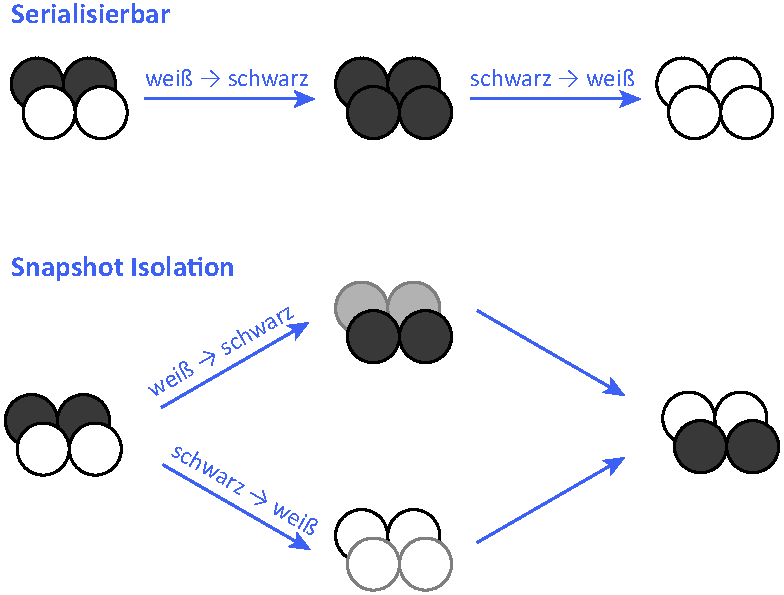
\includegraphics[width=0.8\columnwidth]{img/write_skew.pdf}
	\caption{Beispiel für das Problem des Write Skew bei der Snapshot Isolation \cite{write_skew}}
	\label{fig:write_skew}
\end{figure}

Dabei wird wie in Abbildung \ref{fig:write_skew} dargestellt über Kreuz auf Werte zugegriffen, wodurch ein anderes Ergebnis eintreten kann als bei dem korrespondierenden seriellen Plan.
Im Beispiel gibt es eine Transaktion, welche alle weißen Kugeln schwarz färbt und eine andere Transaktion, welche alle schwarzen Kugeln weiß färbt.
In einem seriellen Plan würden zunächst alle weißen Kugeln schwarz gefärbt, wodurch sämtliche Kugeln schwarz gefärbt wären.
Daraufhin würden alle Kugeln von der anderen Transaktion weiß gefärbt werden, was dazu führen würde, dass sämtliche Kugeln dieselbe Farbe hätten.
Bei Verwendung der Snapshot Isolation würden die Transaktionen gegebenenfalls parallel laufen, was dazu führen würde, dass jede Transaktion den Anfangszustand der Kugeln sehen würden, woraufhin jede Transaktion die für sie relevante Hälfte der Kugeln umfärben würde.
Nach dem Commit beider Transaktionen wäre nun immer noch die Hälfte aller Kugeln weiß und die andere Hälfte schwarz, die Kugeln hätten nur ihre Farbe getauscht, was bei einem seriellen Transaktionsplan nicht auftreten könnte.

\textbf{Serializable Snapshot Isolation (SSI):} Durch den geschickten Einsatz von Sperren, wird das Auftreten der vorhergehen vorgestellten Problematik bei der Snapshot Isolation verhindert.
Somit sind bei der Verwendung dieses Verfahrens keinerlei Abhängigkeitszyklen möglich.

\textbf{Optimistic Concurrency Control (OCC):} Zu guter Letzt soll noch das üblicherweise in Silo verwendete CC-Verfahren untersucht werden, welches eine Variante der Optimistic Concurrency Control darstellt, weshalb es im Folgenden als OCC bezeichnet wird.
Dieses Verfahren sichert ebenfalls die Serialisierbarkeit des Plans und verspricht einen hohen Durchsatz sowie gute Skalierbarkeit.
Weitere Informationen zu Optimistic Concurrency Control und der in Silo implementierten Variante finden sich in \cite{Kung:1981} und \cite{Tu:2013}.

\subsection{Der TPC-C Benchmark}
Um die Geschwindigkeitsvorteile des Serial Safety Nets gegenüber den klassischen Verfahren quantifizieren zu können, wurde der TPC-C Benchmark verwendet.\cite{tpcc}
Es handelt sich dabei um einen Online-Transaction-Processing(OLTP)-Benchmark, welcher mehrere Transaktionstypen und eine komplexe Datenbank bietet.
Die insgesamt fünf verschiedenen Transaktionsarten modellieren dabei die Alltagsaktivitäten eines Großhandels, was das Verwalten und Ausliefern von Bestellungen, das Überwachen von Zahlungen, das Abfragen des Bestellstatus und das Beobachten des Warenbestandes umfasst.
Damit stellt dieser Benchmark eine hervorragende Simulation von stark verbreiteten Anwendungsgebieten dar, welche die Performanz des getesteten Systems in vielen Alltagssituationen einschätzen lässt.
Obwohl in dem Artikel, auf den sich diese Ausarbeitung bezieht \cite{Wang:2015} lediglich der TPC-C Benchmark betrachtet wird, ist hier anzumerken, dass die Autoren in ihrem weiterführenden Artikel \cite{WangJFP16} außerdem den TPC-CC und TPC-EH Benchmark verwendet haben um die Ergebnisse zu bestätigen.

\subsection{Testsystem}
Der Vollständigkeit halber sei hier noch erwähnt, dass zum Durchführen der Tests ein Server mit vier Sockeln verwendet wurde, der mit vier Intel Xeon E7-4807 Prozessoren bestückt war und somit über insgesamt 24 physikalische Rechenkerne verfügte.
Außerdem war das System mit 64GB Hauptspeicher ausgestattet, wodurch es sich um einen mittelgroßes Gerät handelt, wie man es beispielsweise in einem mittelständischen Unternehmen finden würde.
